\documentclass[a4paper]{article}

%% Language and font encodings
\usepackage[spanish]{babel}
\usepackage[utf8x]{inputenc}
\usepackage[T1]{fontenc}

%% Sets page size and margins
\usepackage[a4paper,top=3cm,bottom=2cm,left=3cm,right=3cm,marginparwidth=2cm]{geometry}

%% Useful packages
\usepackage{amsmath}
\usepackage{graphicx}
\usepackage[colorinlistoftodos]{todonotes}
\usepackage[colorlinks=true, allcolors=blue]{hyperref}



\title{Nuestro maravilloso trabajo para la asignatura de\\
Procesamiento de Imágenes Digitales}
\author{U. Autora, O. Autor}

\begin{document}
\maketitle

\begin{abstract}
 \noindent El resumen debe tener como máximo 250 palabras y ser un único párrafo. El resumen debe describir lo más fielmente posible el trabajo realizado (no el propuesto inicialmente, que podría ser distinto). 
 En esta plantilla se presentan las indicaciones para realizar el trabajo de PID, al mismo tiempo que la estructura que debe tener la documentación a presentar. 

\hspace{1cm}

\noindent \textbf{Palabras clave:} 
%(hasta cinco palabras que clasifiquen el trabajo) 
PID, instrucciones, trabajo en grupo, imagen digital.
\end{abstract}


\section{Introducción}

El trabajo de PID debe ser un trabajo de {\bf 70 horas por persona}, que sirva para profundizar en algunos aspectos del procesamiento de imágenes {\bf no vistos en clase}. Se debe trabajar sobre un tema concreto de procesamiento de imágenes {\bf apoyándose en artículo(s) de investigación} relativamente reciente(s) o en {\bf capítulos de libros científicos}.

El objetivo de los trabajos dirigidos consiste en explicar algún método o algoritmo de procesamiento de imágenes de una forma {\bf didáctica}, tanto teóricamente como de forma práctica. Es decir, 
\begin{itemize}
    \item primero, hay que {\bf estudiar el método teórico}, extrayendo las ideas principales de la documentación utilizada, comprendiendo todos los pasos y explicándolos de forma didáctica. Esto significa, por tanto, que {\bf no} debe hacerse una transcripción exacta de lo que aparece en el artículo de investigación referenciado.
    \item Segundo, hay que implementar o {\bf poner en práctica} la implementación existente, también de forma didáctica, tratando de mostrar pasos intermedios, significado de parámetros, experimentando, etc.
    \item Finalmente hay que hacer una {\bf presentación didáctica} del método,  explicando cada uno de los pasos requeridos para llegar al resultado final.

\end{itemize}

Los trabajos se realizarán en grupos de trabajo preferiblemente de tres personas.  A partir de la explicación de las instrucciones del trabajo en grupo, las clases indicadas en el {\bf Calendario} se dedicarán a la realización del trabajo y seguimiento, por parte del profesorado, del trabajo del grupo. 

Se recomienda usar alguna herramienta de planificación y gestión de proyectos para hacer una planificación inicial y un seguimiento posterior del desarrollo del trabajo, registrando las tareas realizadas por cada uno (y el tiempo empleado). Téngase en cuenta que las horas de dedicación de \textbf{cada alumno/a} han de ser \textbf{70 horas}. Será obligatorio presentar los tiempos realizados {\bf individualmente en cada sesión de seguimiento.}

\section{Planteamiento teórico}

La sección \textit{Planteamiento teórico} debe plantear el problema a resolver, así como describir los algoritmos propuestos para su resolución. 

La realización del trabajo está programada en {\bf 4 fases}, cada una de las cuales termina con un {\bf Seguimiento}.
\subsection*{FASE 1}
En la primera fase, \textbf{los miembros del grupo} realizarán la \textbf{propuesta del trabajo dirigido} (TD), acordando con el profesorado el trabajo a realizar. 

Para la búsqueda de libros y bases de datos de revistas, se puede consultar el catálogo fama de la US \url{http://fama.us.es/}. Se recomiendan las bases de datos ScienceDirect (Elsevier), IEEE Xplore y Sringerlink. Si se accede desde fuera de la Universidad, se tendrá que usar el UVUS. Se pueden encontrar recursos para buscar ideas en el documento \textit{Enlaces de interés} del contenido en ev.

Antes de que termine la \textbf{Fase 1}, se debe entregar la {\bf planificación inicial} y la {\bf lista de objetivos} del TD. Se recuerda que en la planificación se debe detallar cómo se distribuirán las {\bf 70 horas/persona} que el grupo debe dedicar al TD, incluidas las sesiones de clase deicadas al trabajo.  
En esta fase debe comprenderse la teoría relativa al trabajo a realizar y quedar perfectamente definido. 

\subsection*{FASE 2}
En esta fase se comenzará a trabajar en la parte práctica y explicación del método. Se recomienda comenzar a escribir la documentación desde el prncipio.

Al finalizar la Fase 2, se mostrará una primera versión de la implementación, algo mínimo. El algoritmo (o algoritmos) a implementar debe estar perfectamente claro y diseñado. 

\subsection*{FASE 3}
En la Fase 3 se seguirá con la realización del trabajo. Al final de la Fase 3, se mostrará una primera versión de la documentación y segunda de la implementación, ahora ya sí, un producto mínimo viable. Se mostrará la hoja de tiempos realizada hasta ese momento y \textbf{ se revisarán los objetivos iniciales} planteados.

\subsection*{FASE 4}
En la última fase se realizará la experimentación para poder evaluar y comparar el método implementado y poder inferir conclusiones. Al final de la Fase 4, se tendrá una primera versión de la presentación (aunque sólo sea un índice), junto con una revisión de la documentación y de la implementación. 

\vspace{1cm}
En la siguiente tabla se resumen los hitos que deben alcanzarse (y entregarse) al final de cada Fase: 

    \begin{center}
    \begin{tabular}{|c||l|}
    \hline
  Seguimiento 1 & Propuesta del TD basándose en una fuente científica.   \\& Planificación inicial y lista de objetivos. \\
  & Estudio y comprensión del método elegido. \\
  & Hoja de tiempos individual.\\
\hline
Seguimiento 2  & Primera versión de la implementación. \\ &  Hoja de tiempos individual.\\
\hline
 Seguimiento 3 & Primera versión de la documentación y segunda de la implementación.\\
&  Hoja de tiempos individual.\\& Revisión de los objetivos. \\
\hline
Seguimiento 4 & Primera versión de la presentación.  \\& Revisión de la documentación  y de la  implementación.\\
\hline
    \end{tabular}
    \end{center}
Los días dedicados a cada Seguimiento aparecen en el Calendario publicado en ev.

\textbf{Todos} los miembros del grupo deberán \textbf{intervenir en la exposición final}, en la que deberán defender su trabajo y comentar los logros teóricos y de implementación obtenidos. Además, deberá hacerse algún ejemplo usando la implementación desarrollada (\textbf{20 minutos en total}). Las exposiciones se realizarán en horario de clase en las dos últimas semanas. Después se abrirá un turno de preguntas.

  %  En la siguiente tabla se muestran las fechas de  \textbf{las exposiciones de cada grupo}. Las exposiones se realizarán en horario de clase.

%\begin{center}
%    \begin{tabular}{|c||r|r|}
%    \hline
%     &Grupos 1,2,3 & Grupos 4,5,6\\
%    \hline\hline
%  Fecha de la exposición & 8 de junio & 9 de junio \\
%\hline
%    \end{tabular}
%    \end{center}

Para la entrega, cada grupo deberá subir, en respuesta a una actividad creada para tal efecto en la ev, los siguientes elementos:

 \begin{itemize}
\item \url{documentacion.pdf}. Consiste en un fichero \url{.pdf} correspondiente a la documentación. 

Estructura de la documentación:

\begin{enumerate}
\item[]  Título
\item[]  Autores
\item[]  Resumen
\item  Introducción 
\item  Planteamiento teórico 
\item  Implementación
\item  Experimentación
\item  (Manual de usuario)
\item  Conclusiones
\item Autoevaluación de cada miembro
\item  Tabla de tiempos
\item[]  Bibliografía
\end{enumerate}

Se puede usar el fichero \url{main.tex} disponible en enseñanza virtual como plantilla de Latex\footnote{Véase el Anexo para algunos apuntes rápidos sobre escritura de textos en LaTex (tomados de \url{Overleaf.com}.}, que es el que se ha usado en este documento. Se recomienda el uso de editores online de LaTeX como \url{Overleaf.com}.

Las referencias se citan así:
bla, bla \cite{clave:revista}, bla, bla \cite{clave:libro}. La bibliografía
debe seguir el estilo de este documento, con las referencias ordenadas alfabéticamente por autores.

También se puede documentar el trabajo en un Notebook de Jupyter, en el que también se puede incluir código LaTex e imprimirlo como pdf.

\item \url{codigo.zip}. Si se ha desarrollado una aplicación propia, debe contener todo el código utilizado, comentado y modulado. Debe contener el ejecutable, si existiera, junto con todos los archivos necesarios para su ejecución de forma que no dé errores de compilación.
Debe contener un {\bf leeme.txt} con instrucciones para ejecutar el código.
Se debe incluir una carpeta \textbf{images} con imágenes de muestra, incluyendo las imágenes usadas en la experimentación.

En lugar de subir el código a la enseñanza virtual, se puede subir a un repositorio y referenciarlo en la documentación. 

En caso de que exista ya una implementación en un repositorio asociado al trabajo escogido, se debe desarrollar una versión propia que incluya explicaciones, paso a paso, ejemplos, modificaciones, etc. Por ejemplo, se puede hacer un notebook de jupyter para esto.



\item \url{presentacion.pdf}. Consiste en un fichero \url{.pdf} con la presentación que se usará en clase para exponer el trabajo.
\end{itemize}

La evaluación del trabajo se realizará en base a una rúbrica que se proporcionará en Blackboard.





\section{Implementación}

Esta sección de la documentación  debe incluir la descripción de la implementación (pero no el código), especificando las tecnologías usadas, el diseño, módulos o partes principales. \textbf{Debe quedar muy claro cuál es la parte original implementada en el programa, qué librerías se han usado y de dónde se han cogido, con referencias apropiadas}. Se debe describir (tanto en la aplicación, como en la documentación, como en la presentación) los pasos seguidos para resolver el problema que se plantea de la forma más divulgativa posible. 

%Se recomienda el uso de Python con la librería \textbf{OpenCV}, \url{https://opencv.org/}.
%Matlab posee también un toolbox de procesamiento de imágenes que se puede usar en los laboratorios de la escuela.
Una opción muy práctica y recomendable es la de usar la librería \textbf{OpenCV} con Python mediante el gestor de paquetes de Anaconda \url{https://www.anaconda.com} y usar los notebook de Jupyter en los que se puede intercalar ejecución de código con explicaciones teóricas. % Éstas sólo son algunas indicaciones. 

Siempre se debe redactar un fichero {\bf Leeme explicando todo lo necesario para poder ejecutar y usar la implementación} en cualquier ordenador (o al menos con el mismo sistema operativo).



\section{Experimentación}

Una sección de ejemplos comentados y pruebas realizadas con el programa desarrollado es imprescindible en este trabajo. Si existen distintos parámetros que intervienen en el método, se deben comprender y experimentar con ellos. También puede ser de interés probar distintos tipos de imágenes dentro del contexto del trabajo. Igualmente importantes (o más) serán las conclusiones que se puedan obtener de la experimentación realizada. 


\section{Manual de usuario}

Se debe incluir un breve manual de usuario en caso de que se desarrolle una aplicación. Si se implementa un notebook de Jupyter, no es necesario un manual de usuario, sino que debe quedar muy guiado, explicando todos los pasos y parámetros.  

\section{Conclusiones}

Se debe introducir una sección de conclusiones que incluyan propuestas claras de mejora o extensión del trabajo (por ejemplo, si no se han podido alcanzar todos los objetivos iniciales). También conclusiones sobre los resultados obtenidos, en qué medida difieren de los esperados. además, son apropiadas conclusiones sobre las desviaciones en cuanto a la planificación inicial, así como conclusiones sobre la experiencia de la realización del trabajo (lecciones aprendidas).

\section{Autoevaluación}

Siguiendo la rúbrica dada, se debe detallar, por parte de  \textbf{cada miembro del grupo}, la puntuación para el trabajo que se considera justa en cada apartado. 

\section{Tabla de tiempos}


Se debe justificar el trabajo realizado por cada componente del grupo, indicando el {\bf tiempo total que cada miembro del grupo ha dedicado} al trabajo (lo que puede implicar diferencia de notas obtenidas por los distintos miembros del grupo). El trabajo realizado debe ser de {\bf 70 horas por estudiante}. Además, debe haber un plan de trabajo \textbf{individual} detallado con las {\bf tareas realizadas por cada miembro} del grupo. Para esto último, se puede usar la tabla siguiente o bien documentos generados por la herramienta de gestión de proyectos que se use, como Projetsii o Microsoft Project, por ejemplo.

\begin{center}
\begin{tabular}{|c|c|c|c|}
\hline
 Fecha de la
 actividad 
& Tiempo (h)
& Miembro
& Actividad realizada
\\\hline
\mbox{ }&\mbox{}&\mbox{ }&\mbox{}\\
\mbox{ }&\mbox{}&\mbox{ }&\mbox{}\\\hline
\end{tabular}
\end{center}


\begin{thebibliography}{10}



\bibitem{clave:libro}
U. N. Experto, \emph{Un libro que escribí},
Editorial, 1996.

\bibitem{clave:revista}
Y. O. Mismo,
``Título del artículo'',
\emph{Revista Publicación Periódica}, Vol. 17, pp. 1-100, 1997.
\end{thebibliography}

\newpage 

\section*{More about how to write an article}
\subsection{How to include Figures}

First you have to upload the image file from your computer using the upload link the project menu. Then use the includegraphics command to include it in your document. Use the figure environment and the caption command to add a number and a caption to your figure. See the code for Figure \ref{fig:frog} in this section for an example.

\begin{figure}[h]
\centering
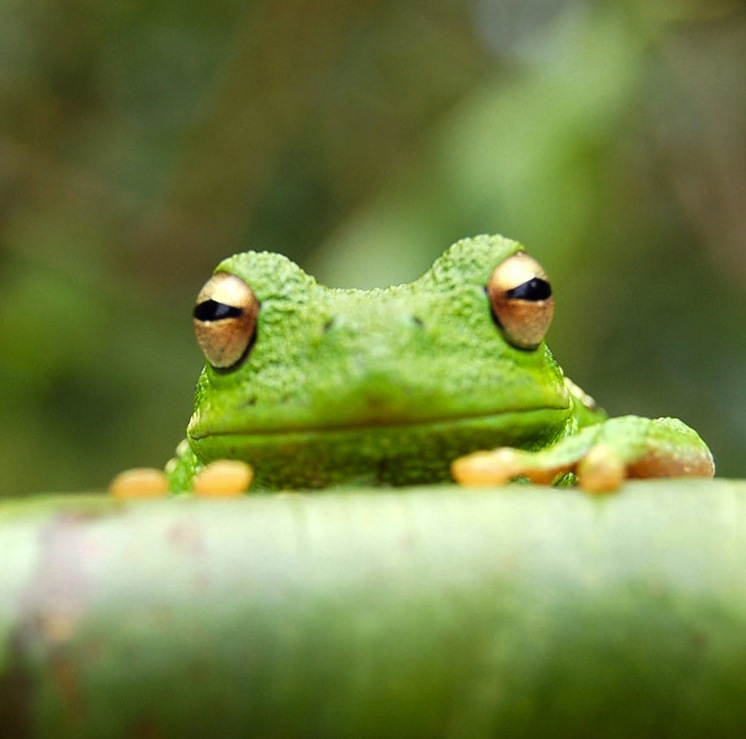
\includegraphics[width=0.3\textwidth]{frog.jpg}
\caption{\label{fig:frog}This frog was uploaded via the project menu.}
\end{figure}


\subsection{How to add Tables}

Use the table and tabular commands for basic tables. See Table~\ref{tab:widgets}, for example. 

\begin{table}[h]
\centering
\begin{tabular}{l|r}
Item & Quantity \\\hline
Widgets & 42 \\
Gadgets & 13
\end{tabular}
\caption{\label{tab:widgets}An example table.}
\end{table}

\subsection{How to write Mathematics}

\LaTeX{} is great at typesetting mathematics. Let $X_1, X_2, \ldots, X_n$ be a sequence of independent and identically distributed random variables with $\text{E}[X_i] = \mu$ and $\text{Var}[X_i] = \sigma^2 < \infty$, and let
\[S_n = \frac{X_1 + X_2 + \cdots + X_n}{n}
      = \frac{1}{n}\sum_{i}^{n} X_i\]
denote their mean. Then as $n$ approaches infinity, the random variables $\sqrt{n}(S_n - \mu)$ converge in distribution to a normal $\mathcal{N}(0, \sigma^2)$.


\subsection{How to create Sections and Subsections}

Use section and subsections to organize your document. Simply use the section and subsection buttons in the toolbar to create them, and we'll handle all the formatting and numbering automatically.

\subsection{How to add Lists}

You can make lists with automatic numbering  or bullet points \dots

\begin{enumerate}
\item Like this,
\item and like this.
\end{enumerate}

\begin{itemize}
\item Like this,
\item and like this.
\end{itemize}

%\subsection{How to add Citations and a References List}

%You can upload a \verb|.bib| file containing your BibTeX entries, created with JabRef; or import your \href{https://www.overleaf.com/blog/184}{Mendeley}, CiteULike or Zotero library as a \verb|.bib| file. You can then cite entries from it, like this: \cite{greenwade93}. Just remember to specify a bibliography style, as well as the filename of the \verb|.bib|.

%You can find a \href{https://www.overleaf.com/help/97-how-to-include-a-bibliography-using-bibtex}{video tutorial here} to learn more about BibTeX.



%\bibliographystyle{alpha}
%\bibliography{sample}

\end{document}